\documentclass[review]{elsarticle}

\usepackage[]{geometry}
\usepackage{amsmath}
\usepackage{tikz}
\usepackage{graphicx}
\usepackage{hyperref}
\usepackage{natbib}
\bibliographystyle{elsarticle-harv}
\biboptions{authoryear}

\newcommand{\ra}{\rightarrow}
\newcommand{\afs}[2]{\Phi_{#1}^{(#2)}}
\newcommand{\Dfrac}[2]{%
  \ooalign{%
    $\genfrac{}{}{1.2pt}0{#1}{#2}$\cr%
    $\color{white}\genfrac{}{}{.4pt}0{\phantom{#1}}{\phantom{#2}}$}%
}
\newcommand{\cond}{\middle\vert}

\newcommand{\sgcomment}[1]{\textcolor{red}{SG: #1}}
\newcommand{\ikcomment}[1]{\textcolor{blue}{IK: #1}}

\journal{Theoretical Population Biology}

\begin{document}
\begin{frontmatter}
  \title{Models of strong selection in large samples}

  \author{Ivan Krukov}
  \author{Simon Gravel}

  \begin{abstract}
    
    Neutral models of genetic diversity tend to be easier to analyze than models with selection.
    Under the neutral Wright-Fisher model, the number of lineages that contribute to ancestry of a
    sample decreases back in time due to coalescent events. As a consequence, useful recursion
    equations can be derived for patterns of polymorphism. By contrast, under negative selection,
    the number of relevant lineages can increase as we go back in time, due to selective deaths. As
    a result, the equivalent recursion equations do not close. However, given a sufficiently large
    sample size, the reduction in the number of lineages due to coalescence is larger than the
    increase in the number of lineages due to selection, and the number of contributing lineages is
    unlikely to increase. We use this observation to derive asymptotically closed recursion
    equations for the distribution of allele frequencies in finite samples. We show that this
    approach is accurate under strong drift and strong natural selection. We derive several
    asymptotic results to determine when the sample size is sufficiently large for drift to
    overcome the effect of selection.
  \end{abstract}

\end{frontmatter}

\section{Introduction}
\label{sec:introduciton}

The allele frequency spectrum (\textit{AFS}) is an important summary of genetic diversity that is
commonly used to infer demographic history and natural selection \citep{}. Given a demographic
scenario of population size histories and migrations, the diffusion approximation or coalescent
simulations can be used to obtain a predicted \textit{AFS} \citep{}. By comparing
predictions to the observed \textit{AFS}, we can compute likelihoods for different demographic
scenarios. Unfortunately, the \textit{AFS} calculations can be time consuming with complex
demographic models, for example with multiple populations with large sample sizes \citep{}.

In the absence of selection, efficient computational shortcuts can be used. In particular, recursion
equations have been derived for moments of the allele frequency distribution
\citep{KimuraCrow1964,Ewens1972,JouganousEtAl2017}. Recently, these recursions have been useful in
fitting complex demographic models to genetic data \citep{JouganousEtAl2017,KammEtAl2017} with
complex demographic models.
 
In the presence of natural selection, the corresponding recursion equations do not close
\citep{Donnelly, JouganousEtAl2017} -- they form an infinite set of coupled ordinary differential
equations. Moment-based closure approximation have been developed \citep{JouganousEtAl2017}, but
these are not robust to strong selection and their convergence properties are not well understood.

Closure of the moment equations under the neutral Wright-Fisher model occurs because the number of
parental lineages that contribute to the present day sample is equal to or smaller than the sample
size. To describe the a sample of size $n$, we need to recursively consider samples of size
$n'\le n$. The decrease in the number of contributing lineages can be framed in terms of coalescent
events \citep{Kingman1982a}. This does not hold under negative selection -- due to selective deaths,
the number of parental lineages $n'$ can be larger than $n$. As we demonstrate later, this leads to
a potentially infinite number of terms in the equations. This is similar to the ancestral selection
graphs (\textit{ASG}), \citep{KroneNeuhauser1997}, where the number of relevant lineages can
increase back in time.

The interplay of drift and selection is important to consider. In large sample sizes, there are many
more common ancestry events than selective deaths, and the number of contributing lineages is
unlikely to increase back in time. This suggests that large sample sizes can lead to
almost-closed recursion equations, as we will demonstrate here.

An additional complication is multiple and/or simultaneous coalescent events -- which emerge with
large sample sizes \citep{BhaskarEtAl2014}. The standard coalescent model only allows one event per
generation, but we also need to consider higher-order events, \textit{e.g.} multiple two-lineage or
three-lineage mergers. These multiple-lineage coalescent events oppose the effect of selection by
rapidly decreasing the number of contributing lineages \citep{NelsonEtAl2019}.

In this article we derive these asymptotically-closed recursions in the Wright-Fisher model, and
study their behavior and applications for modeling the distribution of allele frequencies under
strong selection.

%Unlike the \textit{ASG}, the present method does not need to assume an infinitely large population
%size, and also explicitly tracks multiple coalescent events, which is important with large sample
%sizes \citep{BhaskarEtAl2014}. Our approach can also be combined with the jackknife. Unlike the
%jackknife, our method allows derivation of bounds on the performance of the approximation.

\section{Background}
\label{sec:background}

We consider a haploid Wright-Fisher model of size $N$, focusing on a single biallelic locus. For a
present sample with $n_o$ (offspring) lineages at time $t$, we want to know how many parental
lineages ($n_p$) have been sampled from time $t-1$ (Fig. \ref{fig:schematic}). Under a neutral
coalescent model (Fig. \ref{fig:schematic}A), the number of contributing parental lineages at $t-1$
is $n_p \le n_o$, as the number of lineages decreases due to coalescent events.

To model the interplay of selection and drift, we consider a two-stage selection scheme (Fig.
\ref{fig:schematic}B). First, in a neutral process, $n_p$ parents at $t-1$ produce a (potentially
infinite) number $n_g$ gametes for an intermediate $t-\frac{1}{2}$ generation. Second, the $n_g$
gametes are sampled (with rejection) into $n_o$ offspring at $t$. The number of rejected samples
depends on the strength of negative selection, $s<0$. With stronger negative selection, more gametes
will be rejected, so that $n_o \le n_g$. We want to show that as $n_o$ increases, asymptotically
$n_o \le n_p$.

\begin{figure}[ht]
  \centering
  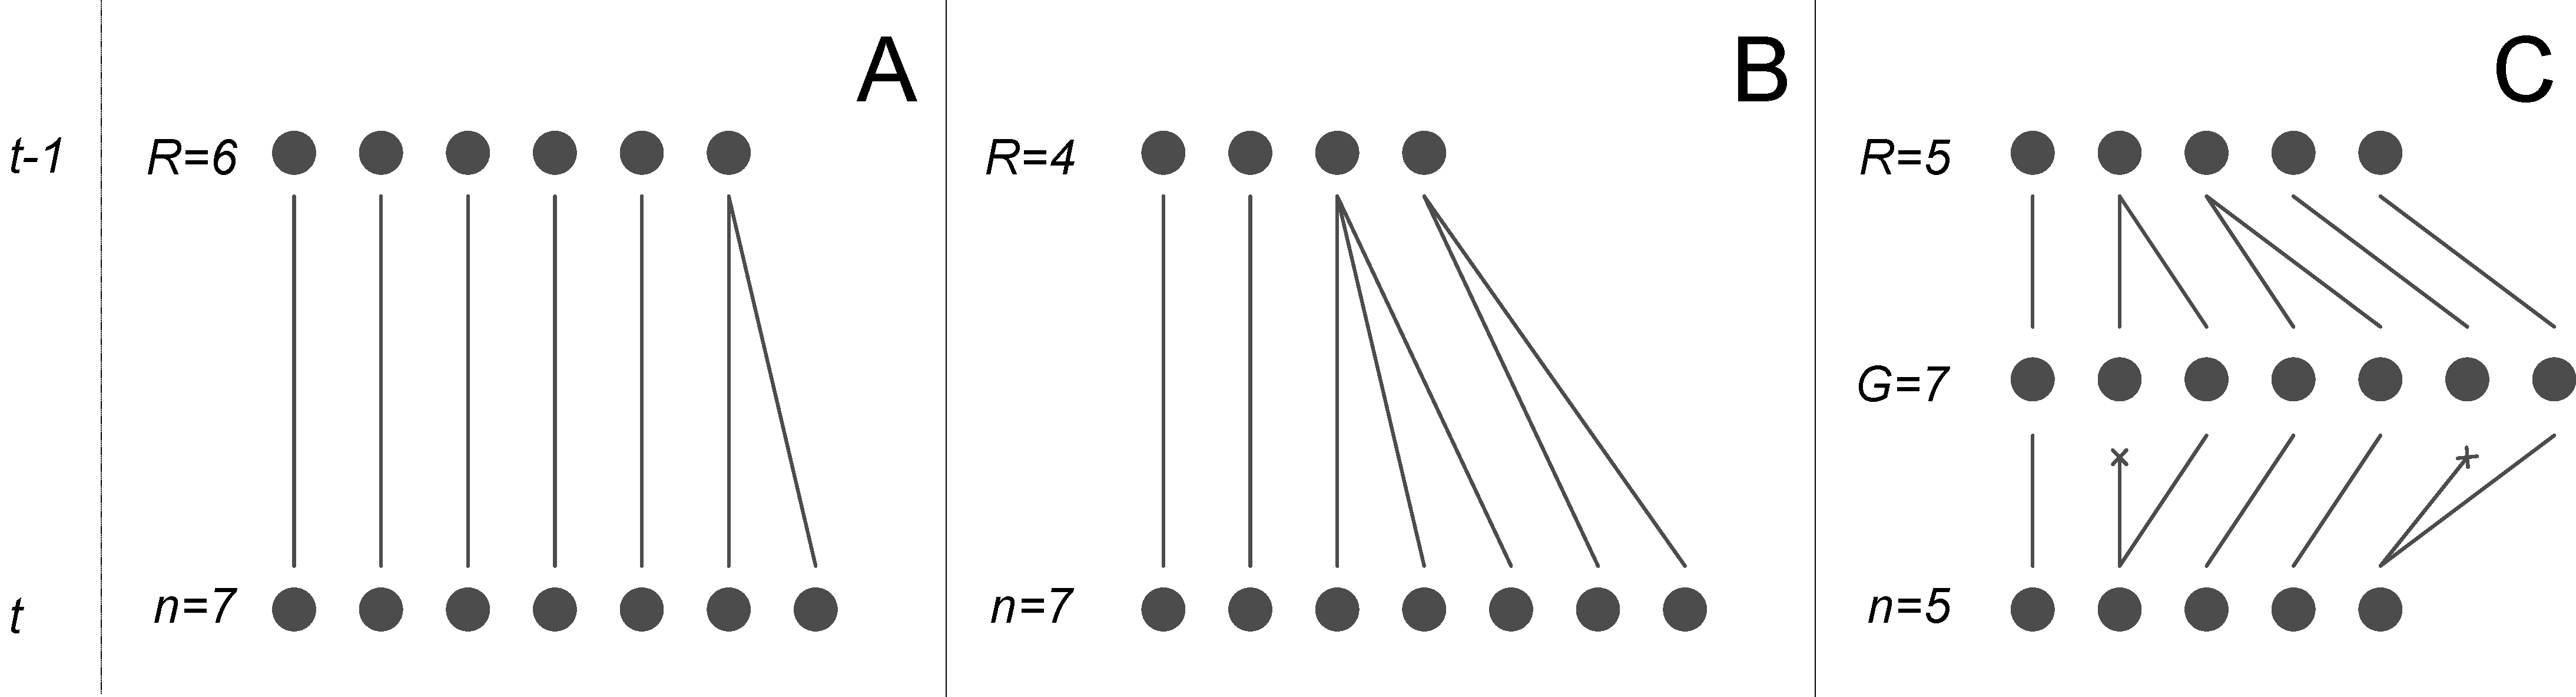
\includegraphics[width=1.0\textwidth]{fig/schematic.pdf}
  \caption{\label{fig:schematic} Realizations of sampling parental lineages under neutrality (A) and
    selection (B). \textbf{A} Under neutrality, possible coalescent events imply that number of
    parental lineages $n_p$ at $t-1$ is less than or equal to $n_o$ offspring lineages at $t$.
    \textbf{B} With selection, we add an intermediate gamete $n_g$ generation at $t-\frac{1}{2}$.
    Production of gametes is neutral, so $n_p\le n_g$. Gametes are sampled with rejection into
    offspring, so $n_o \le n_g$. Rejected samples shown with red crosses. $n_p$ - parental sample
    size (at $t-1$), $n_g$ - number of gametes (at $t-\frac{1}{2}$), $n_o$ - offspring (current)
    sample size (at $t$).}
\end{figure}

In the Kingman coalescent, only a single coalescent event is allowed per generation, in
approximation that sample size is much smaller than the population size: $n_o \ll N$. This implies
that under neutrality $n_p \in [n_o-1, n]$. However, \citet{BhaskarEtAl2014} show that with
increasing sample size, higher order coalescent terms contribute more substantially. This means that
to describe the sample of size $n_o$, we need to consider $n_p$ potentially in the range
$n_p \in [1, n]$. 

We want to describe the time-evolution of the allele-frequency spectrum (\textit{AFS}) in a sample
size $n_o$ at time $t$, which we denote as $\afs{n_o}{t}$. We construct this recursively in terms of
smaller sample sizes, $n'$. In this section, we follow the exposition in \citet{JouganousEtAl2017},
using drift ($\mathcal{D}_{n' \ra n}$) and selection ($\mathcal{S}_{n' \ra n}$) operators. These
operators are sparse matrices that describe changes in allele frequencies in going from sample size
$n'$ to sample size $n$ due to coalescent and selection events, respectively \citep{JouganousEtAl2017}.

Under neutrality (Fig. \ref{fig:schematic}A), we have $n_p \in [1, n_o]$, therefore:

\begin{align}
  \label{eq:op-neutral}
  \afs{n_o}{t} = \sum_{n_p=1}^{n_o}\mathcal{D}_{n_p\ra n_o} \afs{n_p}{t-1}
\end{align}

This equation is closed with respect to the sample size $n_o$. 

To include the effect of selection, we consider first the production of gametes from the parental
generation as a neutral process. Changing the subscripts in \eqref{eq:op-neutral} to refer to
\ref{fig:schematic}B, we have:

\begin{align*}
  \afs{n_g}{t-\frac{1}{2}} = \sum_{n_p=1}^{n_g}\mathcal{D}_{n_p\ra n_g} \afs{n_p}{t-1}
\end{align*}

Then, the produced gametes are sampled with rejection into $n_o$ offspring:

\begin{align*}
  \afs{n_o}{t} = \sum_{n_g=n_o}^{\infty}\mathcal{S}_{n_g\ra n_o} \afs{n_g}{t-\frac{1}{2}}
\end{align*}

Combining the two expressions above, we get:

\begin{align}
  \label{eq:op-selection}
  \afs{n_o}{t} = \sum_{n_g=n_o}^{\infty} \mathcal{S}_{n_g\ra n_o} \sum_{n_p=1}^{n_g} \mathcal{D}_{n_p\ra n_g} \afs{n_p}{t-1}
\end{align}

Since we need to consider a potentially infinite number of gametes produced ($n_g$), the equation
\eqref{eq:op-selection} is no longer closed with respect to sample size.

The number of significant terms in the outer summation depends on the strength of negative selection
$s<0$ -- described here by $\mathcal{S}$. Stronger negative selection will result in more resampling
(Fig. \ref{fig:schematic}B). The number of significant terms in the inner summation, however, depends on
the sample size -- larger sample sizes allow for more coalescent events. Above, this is opaquely
included in $\mathcal{D}$.

\ikcomment{I don't like this explanation, since I feel that the equation doesn't add much to the
  figure.}

We want to show that as the sample size increases, the number of significant terms in
\eqref{eq:op-selection} decreases due to a large number of coalescent events.

The opposing effects of drift and selection on the number of lineages can be clearly seen in the
context of the size of the ancestral selection graph (\textit{ASG}): in which the number of lineages
is described by continuous-time a birth-death process \citep{KroneNeuhauser1997, Wakeley2009}.

\begin{align}
  \label{eq:asg-size}
  n \ra \begin{cases}
    n+1 \hspace{10pt} \text{at rate } \frac{\sigma n}{2} & \text{ (selection) }\\
    n-1 \hspace{10pt} \text{at rate } \frac{n(n-1)}{2}   & \text{ (coalescence) }
  \end{cases}
\end{align}
\ikcomment{The reason I use continuous time rates here is that the coalescent term is obviously
  quadratic in $n$. If I use discrete generations, it will be $\frac{\sigma}{\sigma+n-1}$ for
  selection, and $\frac{n-1}{\sigma+n-1}$ for neutrality, which is a little less obvious.}

where $\sigma$ is a population-scaled selection coefficient. The coalescence term is quadratic with
respect to the sample size $n$, while the selection term is linear. The rate of coalescence is
higher than the rate of selective events if the number of lineages $n>\sigma+1$.

Our goal is to further investigate the interplay of selection and drift, and their effect on the
\textit{AFS}. First, we propose a construction that allows us to calculate the \textit{AFS} under
strong selection and large sample size, accounting for high-order coalescent terms. Second, we show
that with increasing sample size, the system becomes asymptotically closed. We construct exact and
approximate probability distributions that describe the number of contributing lineages.
Additionally, we derive a normal approximation that allows us to calculate the quantile function of
the sample size for a desired degree of closure.


\section{Results}
\label{sec:results}

\subsection{Markov process construction}
\label{subsec:markov}

An alternative way to describe the time-evolution of the \textit{AFS} \eqref{eq:op-selection}, is to
consider a single transition-probability matrix, $\mathbf{P}$, that describes the change due to
drift and selection as a single term, and explicitly models derived and ancestral states:

\begin{equation}
  \label{eq:app:time-evolution}
  \afs{n_o}{t} = \mathbf{P} \afs{n_o}{t-1}
\end{equation}


\ikcomment{$n_o$ and $n$ (without subscript) are the same thing. I use $n_o$ explicitly everywhere,
  but I can probably drop the subscript when it's clear from context.}

$\mathbf{P}$ is a square $n_o \times n_o$ matrix, and it enumerates the number of derived alleles
($i$) at a biallelic locus in a sample of size $n_o$. $\mathbf{P}$ includes contributions from
all possible configurations of parents $n_p$, weighted by the probability of the relevant
coalescent/selective event. We will need to keep track of sample size and number of derived alleles
in the offspring ($o$) and parents ($p$) lineages for a given generation. For example, we use
$\Dfrac{i_p}{n_p}$ (read as ``$i_p$ out of $n_p$'') to denote a sample of size $n$ with $i$ derived in
the parental generation (at $t-1$).

Instead of using the summation formulation presented in \eqref{eq:op-selection}, we use recursive
conditional probabilities, where transitions are defined in terms of transitions in smaller
sample sizes. Each entry of the matrix, $\mathbf{P}_{(i_o,i_p)}$ is a a transition probability from
$i_p$ to $i_o$ derived alleles with sample sizes $n_p$ and $n_o$, respectively. The key observation
is that to construct such probabilities, we can condition on a set of coalescent events
$\{\Lambda\}$ in a smaller sample size:

\begin{align*}
  \mathbf{P}_{(i_o,i_p)} &= P\left[\Dfrac{i_o}{n_o} \cond \Dfrac{i_p}{n_p}\right] \\
  &= \sum_{\lambda\in\{\Lambda\}}P(\lambda)
  P\left[\Dfrac{i_o}{n_o} \cond \Dfrac{i_p}{n_p},\lambda\right] \\
  &= \sum_{\lambda\in\{\Lambda\}}P(\lambda)
  P\left[\Dfrac{i_o-|\lambda|_{i_o}}{n_o-|\lambda|_{n_o}} \cond \Dfrac{i_p-|\lambda|_{i_p}}{n_p-|\lambda|_{n_p}}\right]
\end{align*}

Above, $|\lambda|$ denotes the size of the coalescent event. The third equality ascertains that
conditioning on a coalescent event is equivalent to subtracting relevant lineages from the sample.
This yields a recurrence where transition probabilities in a sample of size $n$ can be
described recursively in terms of transition probabilities in smaller sample sizes, $n' \in [1, n-1]$.

The full derivation of $\mathbf{P}$ for neutral and $\mathbf{P}_s$ for selective cases can be found
in the appendix. This involves enumerating all the coalescent and selective events between samples of
different sizes. We avoid it here for brevity.

Similar to \eqref{eq:op-selection}, the transition probability matrix with selection
($\mathbf{P}_s$), involves considering a large number of intermediate lineages. In practice, we
limit the number of selective events to at most one per lineage -- which means that the maximum number of
contributing lineages is $2n_o$ -- one selective death for each offspring.

The recursive nature of these calculations makes them relatively inefficient. Using a dynamic
programming algorithm, we implement the construction of the neutral matrix $\mathbf{P}$ in the order
of $O(n^3)$ operations. The selection transition probability matrix $\mathbf{P}_s$ needs $O(n^4)$
operations, due to the need to consider intermediate lineages. The increase in complexity makes this
approach unsuitable for large sample sizes, but we derive several approximations in the following
sections.

\ikcomment{--SNIP--}

To retain the closure property under selection, the Markov process needs to take $2n$ lineages in
the parental generation to $n$ lineages in the present. However, such rectangular transition
probability matrix is not suited for our purposes, since we want to describe the behavior of a
sample with constant size $n$. Instead, we only calculate the \textit{truncated} transition
probabilities for a $n \times n$ matrix $Q$. This means that under very strong selection, some
transitions will be unaccounted for. However, since the total sum of transition probabilities sums
to $1$, we can easily calculate the total missing probabilities. As we show in the rest of this
work, this missing probability tends to $0$ as sample size $n$ increases.


\subsection{Calculation of allele frequency spectra}
\label{subsec:afs}

Once the truncated matrix $Q$ is constructed, it can be used to calculate the allele frequency
spectrum. For the infinite sites model at equilibrium, we can \sgcomment{calculate-approximate} the \sgcomment{equilibrium}\textit{AFS} $\Phi$ as a
solution to a linear system:

\begin{equation}
  \label{eq:sfs-calc}
  \Phi = \Phi Q + n \mu e_1
\end{equation}

where $\mu$ is the per-site mutation rate, and $e_1$ is the first column of the identity matrix of
size $n$. Figure \ref{fig:strong-selection} shows the comparison of the \textit{AFS} calculated from
Equation \eqref{eq:sfs-calc}, the diffusion approximation \cite[eq. 9.23]{Ewens2004}, and the
calculation performed in \texttt{Moments} \citep{JouganousEtAl2017}. Panel A shows a comparison at
$Ns=50$, with the population size ($N=2000$), which is substantially larger than the sample size
($n=200$). There is a small deviation between the approaches at large allele frequencies. At
stronger selection coefficients, \texttt{Moments} suffers from numerical instability, while the
diffusion approximation performs well (not shown \sgcomment{why?}).

If the sample size is the same as the population size ($n=N=200$) (Fig.
\ref{fig:strong-selection}B), the diffusion approximation and \texttt{Moments} perform poorly, while
our approach \sgcomment{no need to make it about ourselves here} remains stable. This is expected, since the diffusion framework does not perform well
if multiple coalescent events contribute \sgcomment{cite bhaskar}. Furthermore, if our sample size is the entire population,
we expect recursion equations to be closed \sgcomment{This deserves more clarification}. To confirm this, we compare our result to the
\textit{AFS} calculated from a whole-population haploid Wright-Fisher model, with $N=200$. (Fig.
\ref{fig:strong-selection}B) shows that our calculation is close to the full Wright-Fisher model.
The discrepancy between the curves is due to a difference in the way the selection coefficients are
calculated \sgcomment{What does that mean?}.

\begin{figure}
  \centering
  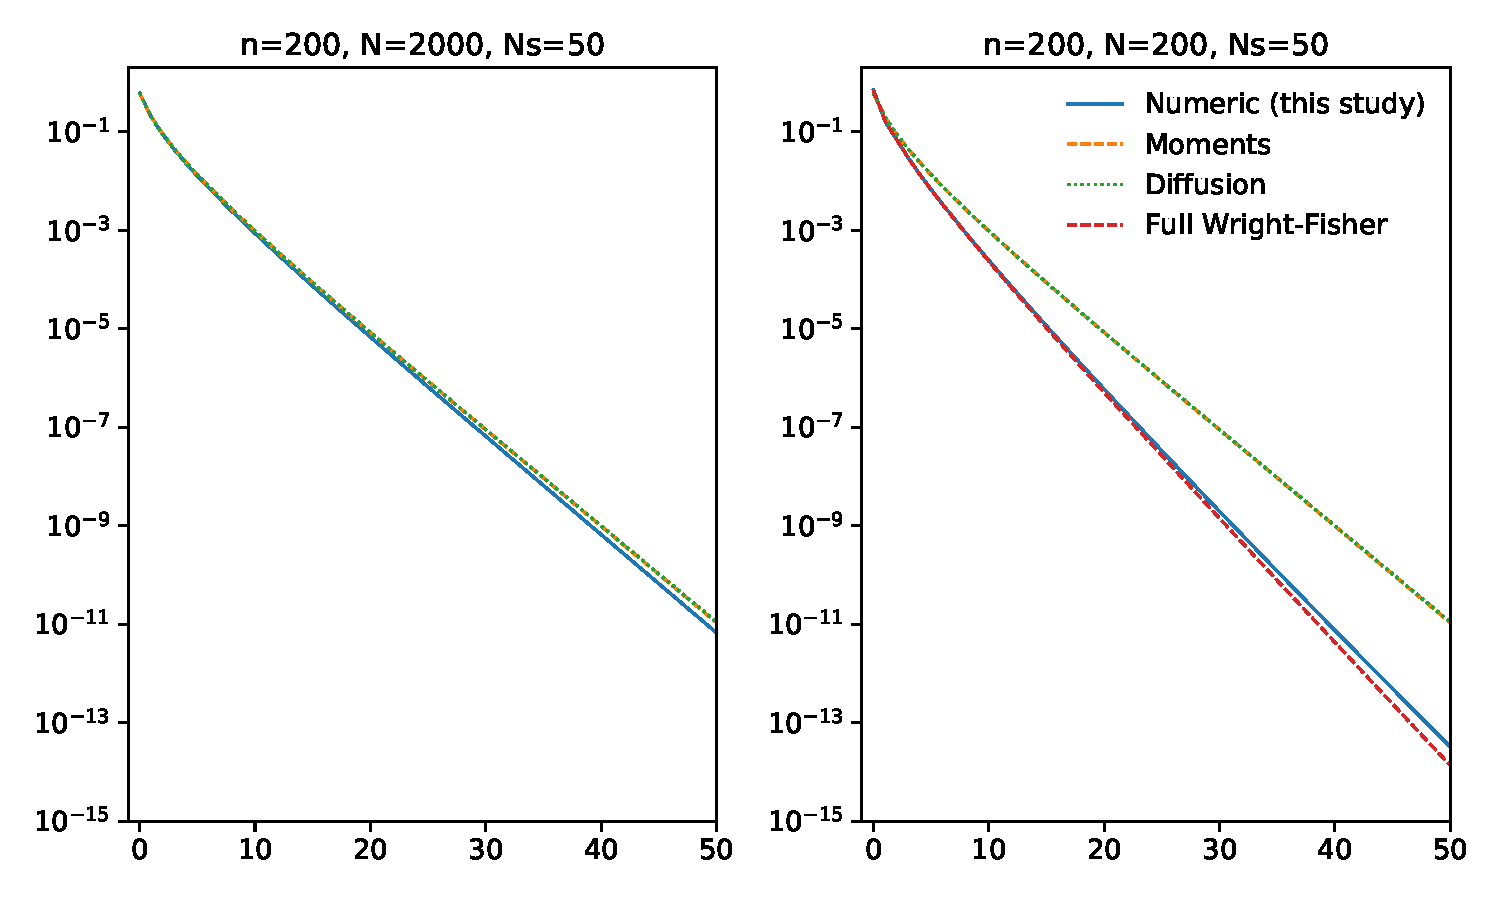
\includegraphics[width=0.7\textheight]{fig/strong_selection.pdf}
  \caption{Normalized allele frequency spectra in a sample of size $n=200$, for highly deleterious
    alleles ($Ns=-50$). (A) shows the frequency spectrum in a sample from a large population
    ($N=2000$), (B) in a small population ($N=200$). Both panels are truncated at $10^{-15}$, to
    show only moderately high allele frequencies.}
  \label{fig:strong-selection}
\end{figure}


\subsection{Closure properties}
\label{subsec:closure}

To \sgcomment{show-investigate} the closure properties of $Q$, we can calculate the total
probability that more that $n$ parental lineages contribute to the sample of a given size. By
construction, the sum of rows of $Q$ should correspond to the total probability mass that included
configurations contribute (Fig. \ref{fig:recurrence} \sgcomment{no figure}). Thus, the probability
that some number of configurations are unaccounted for, with $j$ derived alleles in the parental
sample, is given by $1-\sum_{i=0}^{n}Q_{i,j}$. This probability depends on the number of derived
alleles carried by the parental sample: the more derived alleles, the higher the likelihood of a
selective event. Figure \ref{fig:missing} shows the probability of missing configurations in a
sample size of $n=200$ in the worst-case scenario, with $j=200$ derived lineages.

\begin{figure}
  \centering
  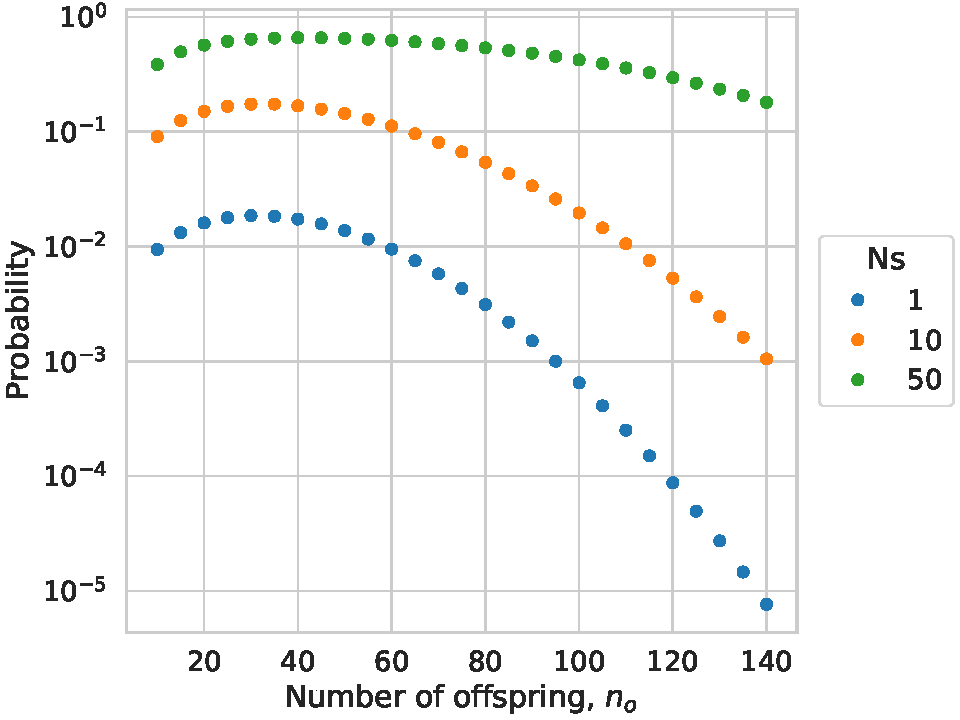
\includegraphics[]{fig/missing.pdf}
  \caption{Probability that unaccounted lineages contribute to the transition probabilities. The
    probabilities are calculated as 1 minus the sum of probabilities for the state where every
    allele is derived. \ikcomment{Need to keep N consistent}}
  \label{fig:missing}
\end{figure}

Since the expected number of drift events increases quadratically and the number of selective events
increases only linearly, the probability that we need additional lineages decreases rapidly with
sample sizes.

\section{Asymptotic closure properties}

We now want to determine what sample size is sufficient so that the number of coalescent events due
to drift is almost always larger than the number of selection events, such that the system remains
closed \eqref{eq:op-selection}. We derive several approximations to the model proposed in the first
section, in order to get a better understanding of this behavior.

As a first order approximation, we consider the mean number of contributing lineages. Then, we
construct a full probability distribution of the number of lineages contributing from the parental
generation. Finally, we propose a normal approximation, which has a simple quantile
function. This allows us to calculate the number of required lineages for the system to be closed
with a given measure of certainty.

In the following derivations, we are assuming that the derived allele is present in the parental
sample at frequency $x$, as opposed to explicitly modeling the count of derive alleles
\ref{sec:markov}, which considerably simplifies the calculations. If we seek the upper bound for the
number of ``lost'' lineages, the maximal value will occur with $x=1$, since only the derived
lineages experience selection.

\subsection{Mean number of contributing lineages}
\label{sec:mean-contr}

For a given sample size, the probability that $n_p$ parents have contributed is:

\begin{align}
  \label{eq:conditional}
  Pr(n_p | n) = \sum_{n_g} Pr(n_p | n_g)Pr(n_g | n)
\end{align}

Where $n_p$ and $n_g$ is the number of contributing parents and gametes, respectively (Fig.
\ref{fig:schematic}C).

Before deriving the distribution formally, we seek to obtain several approximate results.

\subsection{Expected number of lineages used}
\label{subsec:exp-number}

As a first order approximation, we can model $E[n_p | n]$ as the sum of lineages used under drift
$E[n_p | n]$ plus the number of extra lineages required by selection, $E[n_p - n | n]$.

\begin{equation*}
  \begin{aligned}
    \hat{E}[n_p  | n] &= \hat{E}[n_g-n | n] + \hat{E}[n_p | n] \\
    &= N(1-\left( 1 - \frac{1}{N} \right)^n) + n\left( \frac{xs}{1-xs}\right) \\
    &\underset{N\gg n}{\approx} \frac{nxs}{1-xs} - \frac{n^2}{2N}
  \end{aligned}
\end{equation*}

The expectations can be derived directly or from the corresponding probability distributions
\eqref{XX}.The second approximation is made under the assumption that the sample size is much
smaller than the population size. The increase of the number of lineages due to selection is linear.
Drift decreases the number of lineages as a quadratic term with respect to the sample size. This is
analogous to the results from the ancestral selection graph \citep{KroneNeuhauser1997}, eq.
\eqref{eq:asg-size}.

We now want to ask when the expected number of contributing lineages is less that the sample size:

\begin{equation*}
  \begin{aligned}
    \label{eq:critical-sample}
    \hat{E}[n_p | n] &< n \\
    \frac{nxs}{1-xs} - \frac{n^2}{2N} &< n \\
    n &\ge \frac{2Nxs}{1-xs} \\
                                       &\approx 2Nxs
  \end{aligned}
\end{equation*}

This gives a simple expression for the sample size where drift overcomes selection: $n \ge 2Nxs$.
Figure \ref{fig:critical-sample-size} shows this for several selection coefficients, assuming the
entirety of the sample is derived ($x=1$) in a population of $N=1,000$. The $Y$ axis shows the fraction of
contributing parental lineages to the sample size, $\frac{r}{n}$. Above the horizontal line
$\frac{r}{n} > 1$, selection dominates. Below, drift reduces the number of used lineages. The
intercept of the line with $\frac{r}{n} = 1$ is the critical sample size, which is well-approximated
by $2Nsx$.

\begin{figure}
  \centering
  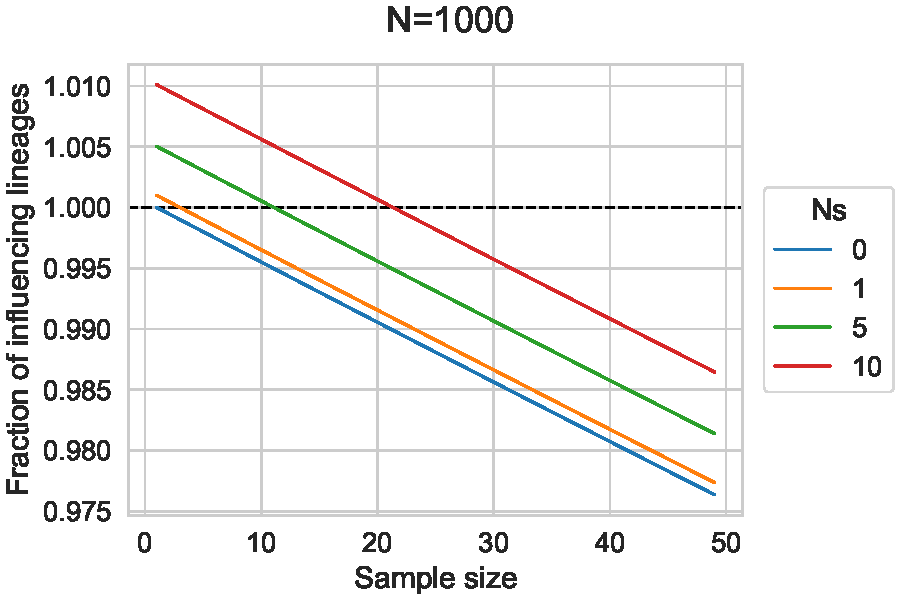
\includegraphics{fig/critical_sample_size.pdf}
  \caption{Critical sample size for different selection coefficients. The $Y$ axis shows the
    fraction of parental lineages over the sample size, $\frac{r}{n}$, each line corresponds to a
    different selection coefficient. Above $\frac{r}{n}\ge 1$, selection dominates, below -- drift.
    The critical sample size, where the expected number of parental contributing lineages is smaller
    than the sample size is well-approximated by $2Ns$.}
  \label{fig:critical-sample-size}
\end{figure}

\subsection{Distribution of number of contributing lineages}
\label{subsec:distribution}

We now construct a probability distribution of the number of contributing lineages one generation
into the past \ref{fig:schematic}C, \eqref{eq:conditional}. 

The number of parental lineages used by drift can be modelled by the modified occupancy
(Arfwedson) distribution \citep{Wakeley2009,ONeill2019,JohnsonEtAl2005}. This is given by:

\begin{align}
  \label{eq:occupancy}
  P(\mathcal{R}=r|\mathcal{G}=g) = \frac{S_2(g,r) N!}{(N-r)! N^g}
\end{align}
where $S_2(g,r)$ is a Stirling number of the second kind, which is the number of ways to partition
$g$ gametes into $r$ parents (see \cite{JohnsonEtAl2005} section 10.4 for a thorough treatment).
Note that the under drift, the number of parents will be smaller or equal to the number of gametes
$r \le g$.

The distribution of the number of gametes, $n_g$ is given by the negative binomial, parameterized by
the total number of trials before $n$ successes:

\begin{align}
  \label{eq:neg-binomial-trials}
  P(\mathcal{G}=g|n) = \binom{g-1}{n-1}(1-xs)^n(xs)^{g-n}
\end{align}

Here, the number of gametes can be larger that the sample size $n \le g$, if selection is present
($s<0$) \sgcomment{Are you not using $s>0$?}.


Combining the two distributions together through \ref{eq:conditional}, we get:

\begin{align}
  \label{eq:lineages-in-past}
   Pr(\mathcal{R}=r|n) = \sum_{g=1}^{\infty} \frac{S_2(g,r) N!}{(N-r)! N^g} \binom{g-1}{n-1}(1-xs)^n(xs)^{g-n}
\end{align}

This distribution does not appear to have a simple analytical form. However, it can be computed
efficiently using methods presented in \citep{ONeill2019}. Figure \ref{fig:sampling-dist} shows the
distribution of the number of contributing parental lineages for several selection coefficients for
a sample $n=20$. In the absence of selection, the distribution has zero probability above $n=20$, as
no extra lineages can be sampled. As the strength of selection is increased, we begin requiring
larger number of lineages.

\begin{figure}
  \centering
  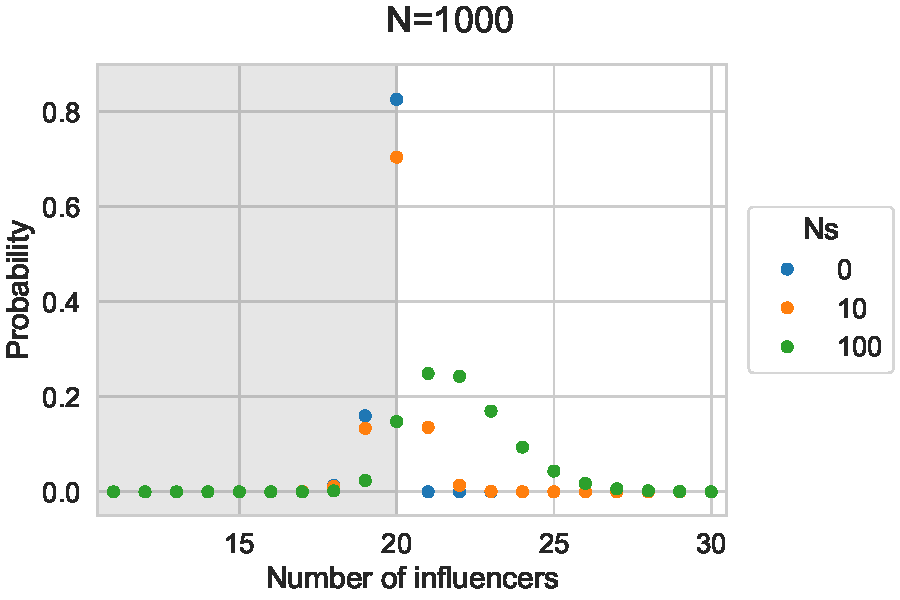
\includegraphics[]{fig/sampling-dist.pdf}
  \caption{The distribution of the number of parental contributing lineages one generation into the
    past ($n=20$, $N=1000$). Shaded area shows the drift-dominated regime, where the number of
    lineages is smaller than the sample size.}
  \label{fig:sampling-dist}
\end{figure}

We defined the critical sample size as $E[n_p | n] = n$. However, the distributions in \ref{fig:XX}
show that there is a large probability that $n_p>n$ at $n_{crit}=2n=20$. In order to guarantee that
drift will out-pace selection, we can calculate the cumulative distribution - Figure
\ref{fig:cumulative-dist}. This shows that a sample size in which the majority of lineages are
accounted for can be substantially larger than the critical sample size of equation
\eqref{eq:critical-sample}. To derive a convenient analytical approximation, we turn to the normal
approximation in the next section.

\begin{figure}
  \centering
  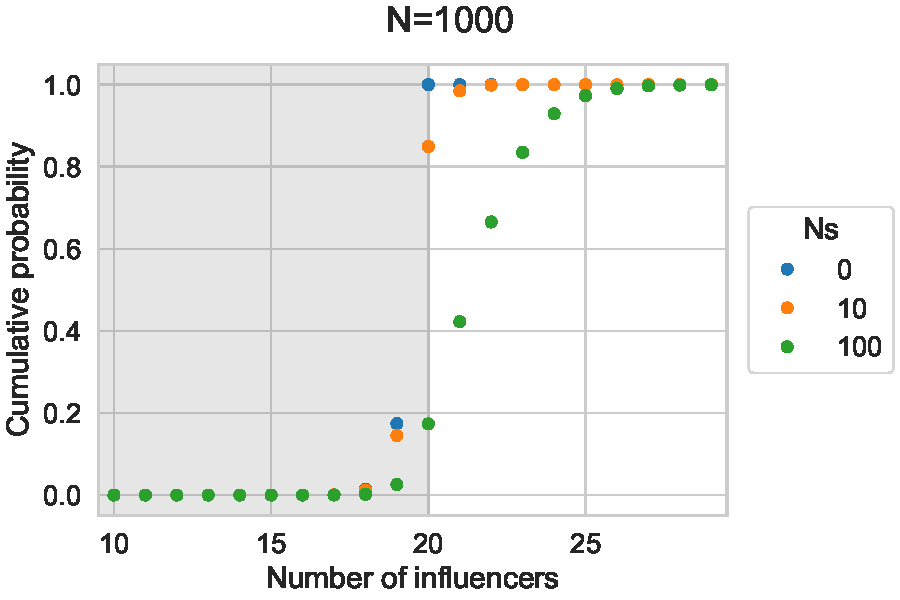
\includegraphics[]{fig/cumulative-dist.pdf}
   \caption{The cumulative distribution of the number of parental contributing lineages one generation into the
    past ($n=20$, $N=1000$). Shaded area shows the drift-dominated regime, where the number of
    lineages is smaller than the sample size. \ikcomment{This should be a two-panel with the
      previous figure}}
  \label{fig:cumulative-dist}
\end{figure}

\subsection{Normal approximation}

Finally, we can construct a normal approximation to the distribution of the number of contributing
lineages. The occupancy distribution is approximated by the normal \citep{ONeill2019} when $n \ll N$.
Likewise, the number of failures (eq. \eqref{eq:neg-binom-fail}) before a given number of successes,
can be approximated by the normal distribution. In the case of large population size, as required by
the approximation of the occupancy by the normal, we can approximate the total number of
contributing lineages as the sum of lineages contributed by the two distributions \sgcomment{What does that mean? Why do you need an approximation? Were you not computing a bound?}. The random
variable which is a sum of two normally-distributed random variables is also normal, with
$\mu=\mu_1+\mu_2$ and $\sigma^2 = \sigma^2_1 + \sigma^2_2$. By combining the required expectations
and variance, we find that the normal approximation then has the form:

\begin{align}
  \label{eq:normal-approximation}
  Pr(\mathcal{R}=r|n) \approx \mathcal{N}( \mu &= \left[(s n)/(1 - s) + N (1 - (1 - 1/N)^n)\right],\\
  \sigma &= \sqrt{N \left((N-1) \left(1-\frac{2}{N}\right)^n+\left(1-\frac{1}{N}\right)^n-N\left(1-\frac{1}{N}\right)^{2 n}\right)+\frac{n s}{(1-s)^2}})
\end{align}

\sgcomment{Tell people N to make self contained} Figure \ref{fig:normal-approximation} shows the quantiles of the normal approximation. We see that
up to $99\%$ of the lineages will be contained within the sample of 200 with $Ns=20$. Larger
percentiles will require larger sample sizes.

\begin{figure}
  \centering
  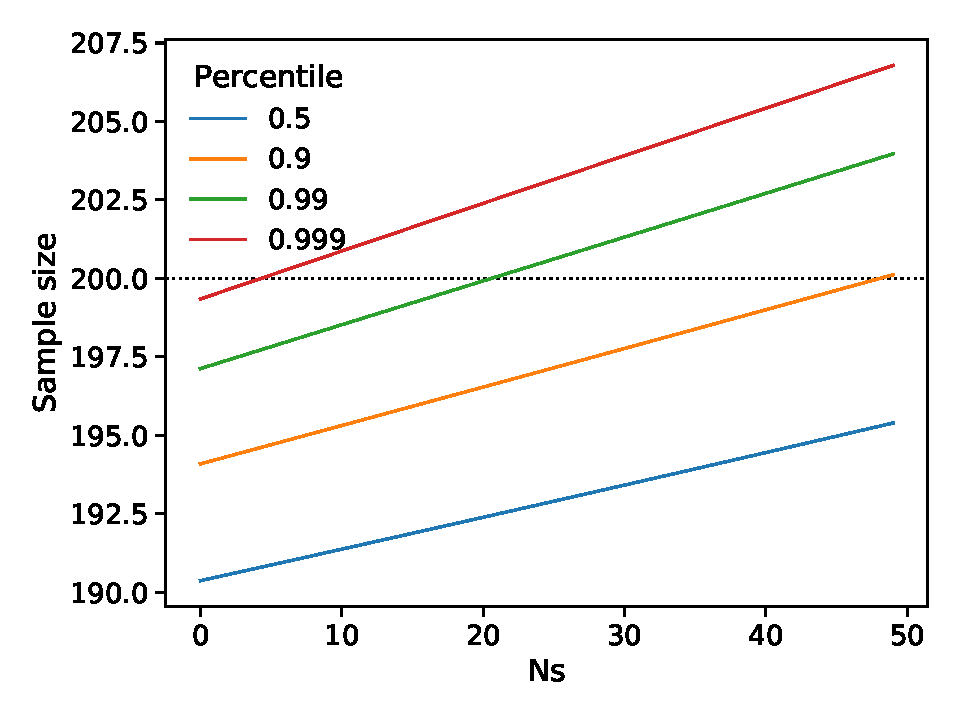
\includegraphics[]{fig/quantile.pdf}
  \caption{The quantile function of the closure of the sample \sgcomment{What is that?}. Each line
    corresponds to different percentile of the normal approximation. Black dashed line shows the
    reference sample size $n=200$ \sgcomment{does it play a special role? If not why mention it (or
      have this line, really)?}. \sgcomment{It also seems like showing the cumulative distributions
      themselves would be more intuitive. E.g $\log(missing p)$. Also would be nice to have the
      numerical calculation. Could you get the cumulative distribution for the occupancy
      distribution from the Oneil algo? }}
  \label{fig:normal-approximation}
\end{figure}


\section{Conclusion}
\label{sec:conclusion}

Classically, the coalescent considers models in the absence of natural selection. Since selection
can increase the number of contributing lineages back in time, the coalescent can no longer be
represented by trees, but instead acquires a graph structure. The ancestral selection graphs
\citep{KroneNeuhauser1997} deal with this in the limit of large population size ($N$).

The large population size approximation implies that the sample size $n$ is much smaller than the
whole population ($n \ll N$), so it is unlikely that more than one coalescent event will happen per
generation. However, recent work \citep{BhaskarEtAl2014,NelsonEtAl2019} pointed out that this
assumption is unreasonable with sample sizes pertinent to modern experiments. As a results, models
that consider multiple coalescent events per generation are gaining increased relevance in the
field \citep{FlemmingtonVoitCoalescentPapers}.

In this work we show that increasing the sample size has another unexpected consequence. As sample
size increases, the larger number of lineages needed due to selection can be masked by coalescent
events. In this sense, the large sample size rescues the model from effect of selection. This means
that recursion equations needed to calculate sample properties are asymptotically closed with large
population size.

At first approximation, $2Nsx$ is a critical sample size, where the decrease of lineages due to
coalescent back in time out-competes the increase due to selection (eq. \eqref{eq:critical-sample}).
Further, we derive the full probability distribution for the number lineages needed with given
selection coefficient and sample size (eq. \eqref{eq:lineages-in-past}). Unfortunately, the
distribution does not have a closed form, so we derive a normal approximation to the number of
lineages that contribute to a sample (eq. \eqref{eq:normal-approximation}). The normal approximation
then allows us to get a quantile function that we use to find if the model preserves closure with
some confidence level.

This work has several implications. First, we can combine the model described here with the
jackknife approximation \citep{JouganousEtAl2017}. This will allow us to construct a more robust
inference framework that can account for large sample size and strong selection.

Further, the results here suggest that effect of weak selection may be detectable in studies with
large sample sizes. This may open up a way for new investigations of natural selection in population
genetics.

\bibliography{disco}

\end{document}
